\section{Results}

\subsection{Single-shot model performance}
% How did we come up with linear models:
% 	- compare performance of all models by "recall"
% 	- compare time with the actual docking time
% 	- test effects of normalization

In order to select most promising models for active-learning iterations, we first compared them on a single batch (figure \ref{fig:fig_4}). 

First, we selected diverse regression models (figure \ref{fig:fig_4}, first row), and compared them with lower-bond and upper-bond baselines. Namely, we trained the regression models to predict the docking score directly, then selected top-1\% from the sorted list as model's hits, and compared model's hits with actual top-1\% of the list. Lower-bond baselines included sklearn's DummyRegressor, as well as custom models yielding random score from either normal or uniform distribution, matching original distribution of scores (RandomUniform and RandomGaussian regressors, respectively). For upper-bond baseline, we used docking scores, provided by the second run of Molsoft's ICM (figure \ref{fig:fig_1}) without fixing a seed value.

For more complicated models such as random forest and decision tree regressors, an increase in prediction quality with increase of model training size. 

As shown in figure \ref{fig:fig_4}, both on retrospective data \cite{ultralarge_docking_first} and data present in this paper, different models show comparable recall, that also becomes more reproducible with the increase of the train size dataset. Expectedly, more complex models such as RandomForestRegressor show superior performance compared to more simple models, albeit at the expense of the significantly increased training and inference time (up to 3 orders of magnitude). Note that here the train dataset size and inference size are related as 4:1 due to 5-fold validation (see \ref{subsec:prediction}). 

Paragraph about effect of normalization

\begin{figure}[h]
% Fig 4: selection of the best single model
% 	- A: model performances
% 	- B: model timing
% 	- C: time vs performance distribution + actual docking time cutoff
\centering
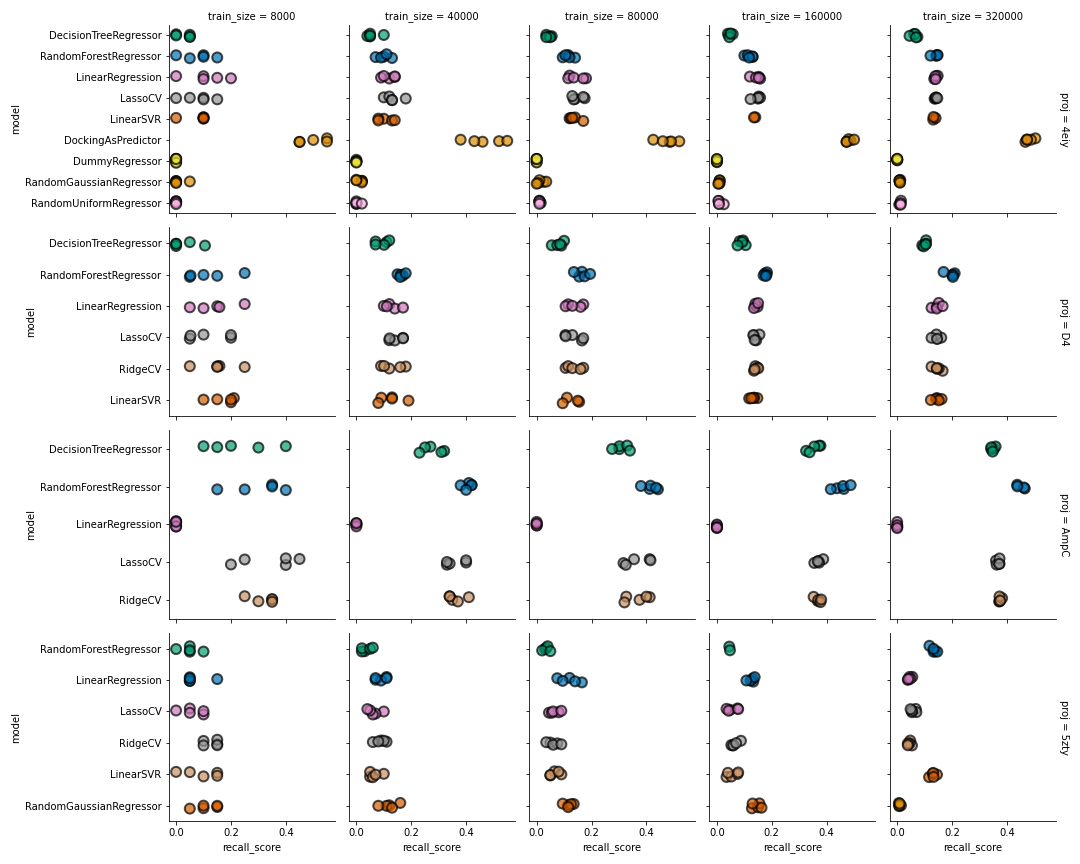
\includegraphics[width=0.8\textwidth]{figures/Figure_4.png}
\caption{Model performance for multiple regression models and their baselines on 4 datasets present in the study. \texttt{recall\_score} shows the share of interception of top-1\% of the regressor's predictions with the actual top-1\%, sorted by docking score}
\label{fig:fig_4}
\end{figure}

\subsection{Optimization of active learning regime}

% How did we come up with iterations scheme:
% 	- compared different train sizes
% 	- compared different regimes (add/noadd)
% 	- compared different ensembling methods
% 	- compare with "docking-as-predictor"

\begin{figure}[h]
% Fig 5: fine-tuning metaparameters of "iterations" 
% 	- batch size effect on the iterations performance
% 	- add/noadd & different ranking schemes effect
% 	- comparison  of the best model with with docking-as-predictor
% 	- TODO: comparison with the really best single model
\centering
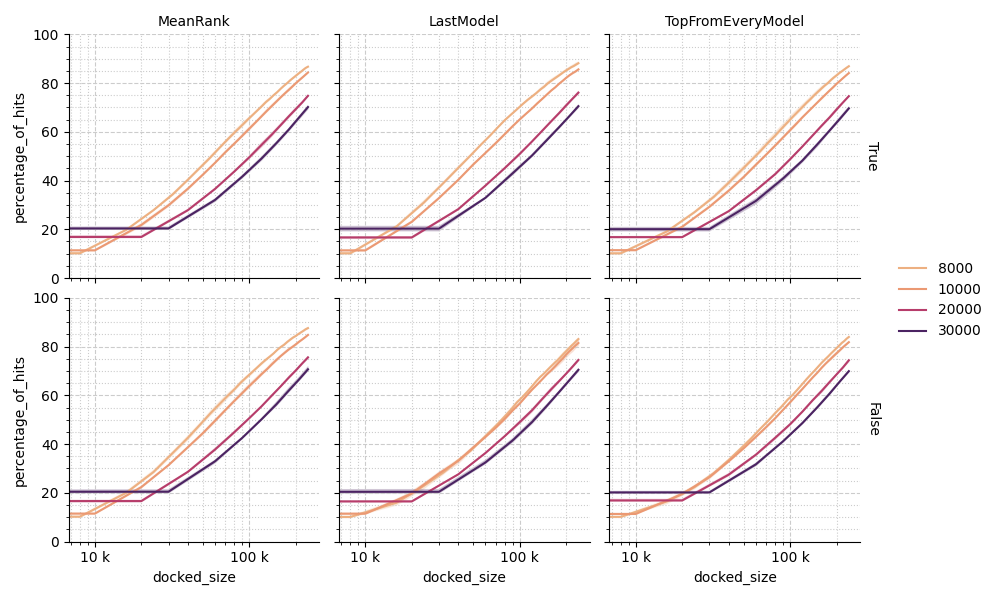
\includegraphics[width=0.8\textwidth]{figures/Figure_3_D4.png}
\caption{Model performance in active learning regime}
\label{fig:fig_3}
\end{figure}

